\linespread{1.5}
Um corpo de massa constante \textit{m} é projetado para fora do planeta Terra numa direção perpendicular à superfície da Terra, com uma velocidade inicial $v_o$. Assumindo que não haja resistência do ar, mas levando em conta a varição do campo gravitacional da Terra com a distância, pede-se
\begin{figure}[H]
    \centering
    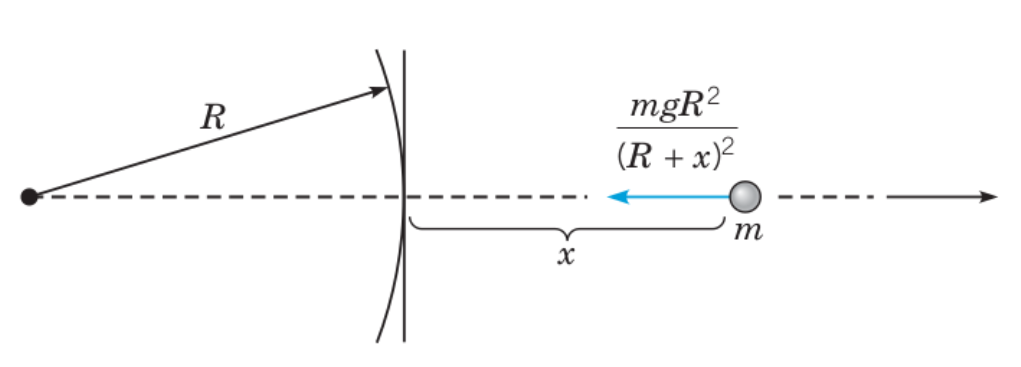
\includegraphics[width=0.7\linewidth]{fig/edo24.png}
    \caption{Corpo atraído pelo campo gravitacional da Terra, em direção ao centro do planeta.}
    \label{fig:edo24}
\end{figure}

\begin{itemize}
    \item[\textbf{a)}] Determine uma expressão que descreva a velocidade do corpo no movimento subsequente à projeção;
    \item[\textbf{b)}]Determine a velocidade inicial necessária para elevar o corpo a uma altitude máxima $A_{max}$, acima da superfície da Terra;
    \item[\textbf{c)}] Encontre a menor velocidade inicial para a qual o corpo não retornará à Terra.
\end{itemize}